
\documentclass[11pt,a4paper]{article}

\usepackage[margin=1in]{geometry}
\usepackage{amsmath,amssymb}
\usepackage{booktabs}
\usepackage{array}
\usepackage{tikz}
\usepackage[hidelinks]{hyperref}
\usepackage{xcolor}
\usepackage{enumitem}

\title{\textbf{BCJRFormer ASIC Architecture}\\
\large Stage 1: Neural-Network Black-Box Definition}
\author{Taimor Sabek \and Haiel Bader}
\date{\today}

\begin{document}

\maketitle

\section{Goal}

The first architecture step is to define the exact input/output boundary of the
\texttt{BCJRFormer} neural-network model used during inference. At this stage,
the internal transformer datapath is intentionally treated as a black box.

The scope of this document is therefore the software boundary of

\[
\texttt{BCJRFormer.forward}(y,\;padding\_mask)
\]

as implemented in the original BCJRFormer repository.

\section{Inference Boundary in the Repository}

During evaluation, the trainer invokes the model as

\begin{verbatim}
x_pred = self.model(y.to(self.device),
                    padding_mask.to(self.device))
\end{verbatim}

Therefore, the BCJRFormer model has two algorithmic inputs:

\begin{enumerate}[label=\arabic*.]
    \item \texttt{y} -- the windowed representation of the received sequences.
    \item \texttt{padding\_mask} -- identifies padded sequence positions.
\end{enumerate}

The model returns one output:

\begin{enumerate}[label=\arabic*.]
    \item \texttt{x\_pred} -- raw output logits of the BCJRFormer model.
\end{enumerate}

\section{First ASIC Black Box}

For the first ASIC architecture iteration, batch size is fixed to one.

\begin{center}
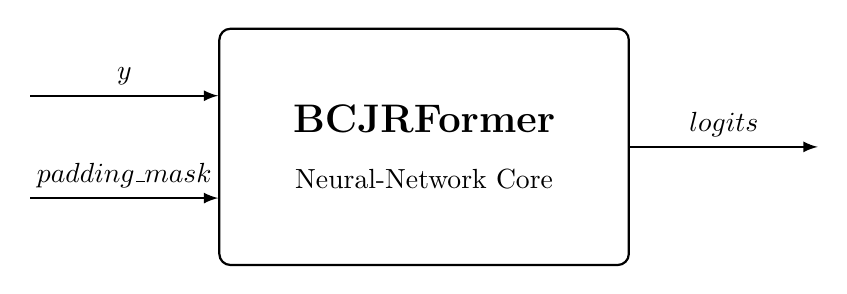
\begin{tikzpicture}[>=latex, thick]
    \node[
        draw,
        rounded corners,
        minimum width=5.2cm,
        minimum height=3.0cm,
        align=center
    ] (model) {\Large \textbf{BCJRFormer}\\[3mm]
               Neural-Network Core};

    \draw[->] (-5.0,0.65) -- (model.west |- 0,0.65)
        node[midway,above] {$y$};

    \draw[->] (-5.0,-0.65) -- (model.west |- 0,-0.65)
        node[midway,above] {$padding\_mask$};

    \draw[->] (model.east) -- (5.0,0)
        node[midway,above] {$logits$};
\end{tikzpicture}
\end{center}

This black box corresponds to the complete \texttt{BCJRFormer.forward()} function,
including the input embedding, positional/sequence embeddings, transformer
encoder, final linear projection, and the sequence-combination operation.

\section{Input 1: Windowed Received Data \texttt{y}}

The dataset first constructs a windowed representation with

\begin{verbatim}
y = self.trellis.get_windowed_version(...)
\end{verbatim}

Before batching, its shape is

\[
[M_{\max},\,N,\,W,\,S]
\]

and after the DataLoader adds the batch dimension,

\[
\boxed{
y \in \mathbb{R}^{1 \times M_{\max} \times N \times W \times S}
}
\]

where:

\begin{table}[h]
\centering
\begin{tabular}{>{\ttfamily}l p{9.5cm}}
\toprule
\textnormal{Parameter} & \textnormal{Meaning} \\
\midrule
M\_MAX & Maximum number of received sequences/transmissions. \\
N & Encoded sequence length / number of transformer positions per received sequence. \\
W & Trellis drift-window size. \\
S & Number of retained trellis-state features per window position. \\
\bottomrule
\end{tabular}
\end{table}

The trellis implementation defines

\[
S = q^{n_v}-1
\]

for the default non-full-state representation, and

\[
\texttt{WINDOW\_BLOCK\_DIM}
    = W \cdot S.
\]

At the beginning of \texttt{BCJRFormer.forward()}, the final two dimensions are
flattened. Thus the effective feature vector presented to the input embedding is

\[
\boxed{
y_{\mathrm{flat}}
\in
\mathbb{R}^{1 \times (M_{\max}N) \times (WS)}
}
\]

before projection to the transformer embedding dimension $d_{\mathrm{model}}$.

\section{Input 2: Padding Mask}

The dataset creates the padding mask from the padded entries of \texttt{y}.
For batch size one,

\[
\boxed{
padding\_mask
\in
\{0,1\}^{1 \times M_{\max} \times N}
}
\]

The model reshapes this mask internally for use by the transformer encoder.

Its purpose is to prevent padded positions, which correspond to unavailable
received sequences, from contributing to the model result.

\section{Output: Raw Logits}

The transformer output is projected by the final linear layer. For the binary
case ($q=2$), the model uses one output channel per encoded position.

After the outputs of the available received sequences are combined, the
BCJRFormer model returns

\[
\boxed{
logits
\in
\mathbb{R}^{1 \times N}
}
\]

for batch size one.

These values are \textbf{raw logits}. They are not yet decoded binary values.

\section{Sigmoid and Hard Decision}

During evaluation, the repository performs

\begin{verbatim}
x_pred = torch.round(torch.sigmoid(x_pred))
\end{verbatim}

\textbf{after} the call to \texttt{BCJRFormer.forward()}.

Therefore, for the first ASIC black box defined in this document,

\[
\boxed{\text{sigmoid and round are outside the BCJRFormer core}}
\]

and the output of the black box remains the raw logit vector.

For a later complete decoder architecture, the binary hard decision can be
implemented without explicitly calculating the sigmoid because

\[
\sigma(x) > 0.5
\iff
x > 0.
\]

Thus,

\[
\operatorname{round}(\sigma(x))
=
\begin{cases}
1, & x > 0,\\
0, & x \le 0.
\end{cases}
\]

This possible hardware optimization is not part of the current black-box
definition.

\section{Generic Architecture Parameters}

The first architecture can therefore be parameterized by:

\begin{table}[h]
\centering
\begin{tabular}{>{\ttfamily}l p{9.5cm}}
\toprule
\textnormal{Parameter} & \textnormal{Description} \\
\midrule
M\_MAX & Maximum number of received sequences. \\
N & Encoded sequence length. \\
WINDOW\_SIZE & Trellis window size $W$. \\
N\_STATE\_FEATURES & Number of state features $S$. \\
WINDOW\_BLOCK\_DIM & Input feature dimension $W \times S$. \\
D\_MODEL & Transformer embedding dimension. \\
NUM\_HEADS & Number of attention heads. \\
NUM\_LAYERS & Number of transformer decoder/encoder blocks used by the model. \\
Q & Symbol alphabet size; the first hardware target is $Q=2$. \\
\bottomrule
\end{tabular}
\end{table}

The concrete values will later be configured to match the trained reference
model and its golden Python results.

\section{Current Black-Box Interface Summary}

For the initial binary, batch-size-one architecture:

\[
\boxed{
\begin{aligned}
y &: [1,M_{\max},N,W,S] \\
padding\_mask &: [1,M_{\max},N] \\
BCJRFormer(y,padding\_mask) &\longrightarrow logits:[1,N]
\end{aligned}
}
\]

The next architecture step is to open this black box and divide
\texttt{BCJRFormer.forward()} into synthesizable sub-blocks, beginning with the
input embedding and transformer encoder.

\section{Repository References}

\begin{itemize}
    \item BCJRFormer repository:
    \url{https://github.com/streit-julian/BCJRFormer}
    \item BCJRFormer model:
    \url{https://github.com/streit-julian/BCJRFormer/blob/main/bcjrformer/models/bcjrformer.py}
    \item Marker trainer / inference path:
    \url{https://github.com/streit-julian/BCJRFormer/blob/main/bcjrformer/trainers/bcjrformer_marker_trainer.py}
    \item Dataset:
    \url{https://github.com/streit-julian/BCJRFormer/blob/main/bcjrformer/datasets/bcjrformer_dataset.py}
    \item Trellis window generation:
    \url{https://github.com/streit-julian/BCJRFormer/blob/main/bcjrformer/trellis.py}
\end{itemize}

\end{document}
